\documentclass{standalone}
\usepackage{tikz}
\usetikzlibrary{patterns, positioning}


\begin{document}
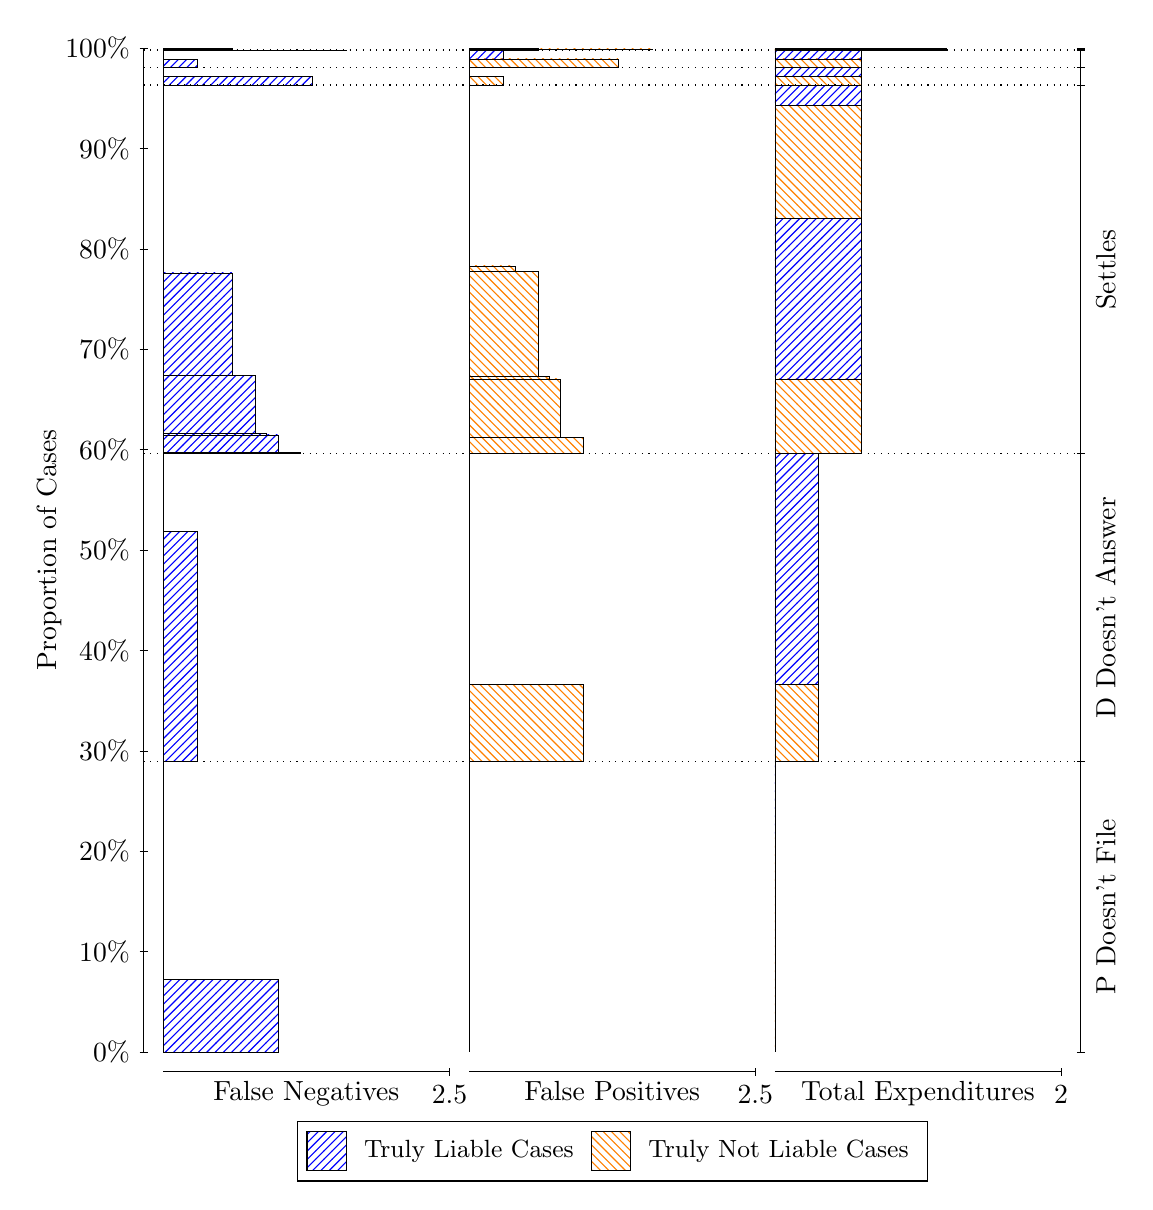
\begin{tikzpicture}
\draw[black, very thin] (1.5,1.75) -- (1.5,14.5);
\node[rotate=90, text=black, anchor=center] at (0.3, 8.125) {Proportion of Cases};
\draw[black, very thin] (1.45,1.75) -- (1.55,1.75);
\node[text=black, anchor=east] at (1.45, 1.75) {0\%};
\draw[black, very thin] (1.45,3.025) -- (1.55,3.025);
\node[text=black, anchor=east] at (1.45, 3.025) {10\%};
\draw[black, very thin] (1.45,4.3) -- (1.55,4.3);
\node[text=black, anchor=east] at (1.45, 4.3) {20\%};
\draw[black, very thin] (1.45,5.575) -- (1.55,5.575);
\node[text=black, anchor=east] at (1.45, 5.575) {30\%};
\draw[black, very thin] (1.45,6.85) -- (1.55,6.85);
\node[text=black, anchor=east] at (1.45, 6.85) {40\%};
\draw[black, very thin] (1.45,8.125) -- (1.55,8.125);
\node[text=black, anchor=east] at (1.45, 8.125) {50\%};
\draw[black, very thin] (1.45,9.4) -- (1.55,9.4);
\node[text=black, anchor=east] at (1.45, 9.4) {60\%};
\draw[black, very thin] (1.45,10.675) -- (1.55,10.675);
\node[text=black, anchor=east] at (1.45, 10.675) {70\%};
\draw[black, very thin] (1.45,11.95) -- (1.55,11.95);
\node[text=black, anchor=east] at (1.45, 11.95) {80\%};
\draw[black, very thin] (1.45,13.225) -- (1.55,13.225);
\node[text=black, anchor=east] at (1.45, 13.225) {90\%};
\draw[black, very thin] (1.45,14.5) -- (1.55,14.5);
\node[text=black, anchor=east] at (1.45, 14.5) {100\%};

\draw[black, very thin] (13.4,1.75) -- (13.4,14.5);
\draw[black, very thin] (13.35,1.75) -- (13.45,1.75);
\node[anchor=west] at (13.35, 1.75) {};
\draw[black, very thin] (13.35,5.4356) -- (13.45,5.4356);
\node[anchor=west] at (13.35, 5.4356) {};
\draw[black, very thin] (13.35,9.3477) -- (13.45,9.3477);
\node[anchor=west] at (13.35, 9.3477) {};
\draw[black, very thin] (13.35,14.03) -- (13.45,14.03);
\node[anchor=west] at (13.35, 14.03) {};
\draw[black, very thin] (13.35,14.251) -- (13.45,14.251);
\node[anchor=west] at (13.35, 14.251) {};
\draw[black, very thin] (13.35,14.467) -- (13.45,14.467);
\node[anchor=west] at (13.35, 14.467) {};
\draw[black, very thin] (13.35,14.483) -- (13.45,14.483);
\node[anchor=west] at (13.35, 14.483) {};
\draw[black, very thin] (13.35,14.5) -- (13.45,14.5);
\node[anchor=west] at (13.35, 14.5) {};

\draw[black, very thin, pattern color=blue, pattern=north east lines] (1.75,1.75) rectangle (3.2033,2.6674);
\draw[black, very thin, pattern color=orange, pattern=north west lines] (1.75,2.6674) rectangle (1.75,5.4356);
\draw[black, very thin, pattern color=blue, pattern=north east lines] (1.75,5.4356) rectangle (2.186,8.3633);
\draw[black, very thin, pattern color=orange, pattern=north west lines] (1.75,8.3633) rectangle (1.75,9.3477);
\draw[black, very thin, pattern color=blue, pattern=north east lines] (1.75,9.3477) rectangle (3.494,9.3676);
\draw[black, very thin, pattern color=blue, pattern=north east lines] (1.75,9.3676) rectangle (3.2033,9.5876);
\draw[black, very thin, pattern color=blue, pattern=north east lines] (1.75,9.5876) rectangle (3.058,9.6058);
\draw[black, very thin, pattern color=blue, pattern=north east lines] (1.75,9.6058) rectangle (2.9127,10.345);
\draw[black, very thin, pattern color=blue, pattern=north east lines] (1.75,10.345) rectangle (2.622,11.643);
\draw[black, very thin, pattern color=orange, pattern=north west lines] (1.75,11.643) rectangle (1.75,14.03);
\draw[black, very thin, pattern color=blue, pattern=north east lines] (1.75,14.03) rectangle (3.6393,14.141);
\draw[black, very thin, pattern color=orange, pattern=north west lines] (1.75,14.141) rectangle (1.75,14.251);
\draw[black, very thin, pattern color=blue, pattern=north east lines] (1.75,14.251) rectangle (2.186,14.357);
\draw[black, very thin, pattern color=orange, pattern=north west lines] (1.75,14.357) rectangle (1.75,14.467);
\draw[black, very thin, pattern color=blue, pattern=north east lines] (1.75,14.467) rectangle (4.0753,14.472);
\draw[black, very thin, pattern color=orange, pattern=north west lines] (1.75,14.472) rectangle (1.75,14.483);
\draw[black, very thin, pattern color=blue, pattern=north east lines] (1.75,14.483) rectangle (2.622,14.495);
\draw[black, very thin, pattern color=orange, pattern=north west lines] (1.75,14.495) rectangle (1.75,14.5);
\draw[black, very thin, pattern color=orange, pattern=north west lines] (5.6333,1.75) rectangle (5.6333,4.5182);
\draw[black, very thin, pattern color=blue, pattern=north east lines] (5.6333,4.5182) rectangle (5.6333,5.4356);
\draw[black, very thin, pattern color=orange, pattern=north west lines] (5.6333,5.4356) rectangle (7.0867,6.4199);
\draw[black, very thin, pattern color=blue, pattern=north east lines] (5.6333,6.4199) rectangle (5.6333,9.3477);
\draw[black, very thin, pattern color=orange, pattern=north west lines] (5.6333,9.3477) rectangle (7.0867,9.5563);
\draw[black, very thin, pattern color=orange, pattern=north west lines] (5.6333,9.5563) rectangle (6.796,10.298);
\draw[black, very thin, pattern color=orange, pattern=north west lines] (5.6333,10.298) rectangle (6.6507,10.334);
\draw[black, very thin, pattern color=orange, pattern=north west lines] (5.6333,10.334) rectangle (6.5053,11.662);
\draw[black, very thin, pattern color=orange, pattern=north west lines] (5.6333,11.662) rectangle (6.2147,11.734);
\draw[black, very thin, pattern color=blue, pattern=north east lines] (5.6333,11.734) rectangle (5.6333,14.03);
\draw[black, very thin, pattern color=orange, pattern=north west lines] (5.6333,14.03) rectangle (6.0693,14.14);
\draw[black, very thin, pattern color=blue, pattern=north east lines] (5.6333,14.14) rectangle (5.6333,14.251);
\draw[black, very thin, pattern color=orange, pattern=north west lines] (5.6333,14.251) rectangle (7.5227,14.361);
\draw[black, very thin, pattern color=blue, pattern=north east lines] (5.6333,14.361) rectangle (6.0693,14.467);
\draw[black, very thin, pattern color=orange, pattern=north west lines] (5.6333,14.467) rectangle (6.5053,14.478);
\draw[black, very thin, pattern color=blue, pattern=north east lines] (5.6333,14.478) rectangle (5.6333,14.483);
\draw[black, very thin, pattern color=orange, pattern=north west lines] (5.6333,14.483) rectangle (7.9587,14.488);
\draw[black, very thin, pattern color=blue, pattern=north east lines] (5.6333,14.488) rectangle (6.5053,14.5);
\draw[black, very thin, pattern color=orange, pattern=north west lines] (9.5167,1.75) rectangle (9.5167,4.5182);
\draw[black, very thin, pattern color=blue, pattern=north east lines] (9.5167,4.5182) rectangle (9.5167,5.4356);
\draw[black, very thin, pattern color=orange, pattern=north west lines] (9.5167,5.4356) rectangle (10.062,6.4199);
\draw[black, very thin, pattern color=blue, pattern=north east lines] (9.5167,6.4199) rectangle (10.062,9.3477);
\draw[black, very thin, pattern color=orange, pattern=north west lines] (9.5167,9.3477) rectangle (10.607,10.298);
\draw[black, very thin, pattern color=blue, pattern=north east lines] (9.5167,10.298) rectangle (10.607,12.335);
\draw[black, very thin, pattern color=orange, pattern=north west lines] (9.5167,12.335) rectangle (10.607,13.772);
\draw[black, very thin, pattern color=blue, pattern=north east lines] (9.5167,13.772) rectangle (10.607,14.03);
\draw[black, very thin, pattern color=orange, pattern=north west lines] (9.5167,14.03) rectangle (10.607,14.14);
\draw[black, very thin, pattern color=blue, pattern=north east lines] (9.5167,14.14) rectangle (10.607,14.251);
\draw[black, very thin, pattern color=orange, pattern=north west lines] (9.5167,14.251) rectangle (10.607,14.361);
\draw[black, very thin, pattern color=blue, pattern=north east lines] (9.5167,14.361) rectangle (10.607,14.467);
\draw[black, very thin, pattern color=orange, pattern=north west lines] (9.5167,14.467) rectangle (11.697,14.478);
\draw[black, very thin, pattern color=blue, pattern=north east lines] (9.5167,14.478) rectangle (11.697,14.483);
\draw[black, very thin, pattern color=orange, pattern=north west lines] (9.5167,14.483) rectangle (11.697,14.488);
\draw[black, very thin, pattern color=blue, pattern=north east lines] (9.5167,14.488) rectangle (11.697,14.5);
\draw[black, dotted] (1.5,5.4356) -- (13.4,5.4356);
\draw[black, dotted] (1.5,9.3477) -- (13.4,9.3477);
\draw[black, dotted] (1.5,14.03) -- (13.4,14.03);
\draw[black, dotted] (1.5,14.251) -- (13.4,14.251);
\draw[black, dotted] (1.5,14.467) -- (13.4,14.467);
\draw[black, dotted] (1.5,14.483) -- (13.4,14.483);
\draw[black, very thin] (1.75,1.5) -- (5.3833,1.5);
\node[text=black, anchor=north] at (3.5667, 1.5) {False Negatives};
\draw[black, very thin] (5.3833,1.45) -- (5.3833,1.55);
\node[text=black, anchor=north] at (5.3833, 1.45) {2.5};

\draw[black, very thin] (5.6333,1.5) -- (9.2667,1.5);
\node[text=black, anchor=north] at (7.45, 1.5) {False Positives};
\draw[black, very thin] (9.2667,1.45) -- (9.2667,1.55);
\node[text=black, anchor=north] at (9.2667, 1.45) {2.5};

\draw[black, very thin] (9.5167,1.5) -- (13.15,1.5);
\node[text=black, anchor=north] at (11.333, 1.5) {Total Expenditures};
\draw[black, very thin] (13.15,1.45) -- (13.15,1.55);
\node[text=black, anchor=north] at (13.15, 1.45) {2};

\node[text=black, centered, rotate=90] at (13.72, 3.5928) {P Doesn't File};
\node[text=black, centered, rotate=90] at (13.72, 7.3916) {D Doesn't Answer};
\node[text=black, centered, rotate=90] at (13.72, 11.689) {Settles};





\draw (7.449999999999999,1.5) node[draw=none] (baseCoordinate) {};
\begin{scope}[align=center]
        \matrix[scale=0.5, draw=black, below=0.5cm of baseCoordinate, nodes={draw}, column sep=0.1cm]{
            \node[rectangle, draw, minimum width=0.5cm, minimum height=0.5cm, pattern color=blue, pattern=north east lines] {}; &
            \node[draw=none, font=\small, text=black] (B) {Truly Liable Cases}; &
            \node[rectangle, draw, minimum width=0.5cm, minimum height=0.5cm, pattern color=orange, pattern=north west lines] {}; &
            \node[draw=none, font=\small, text=black] (B) {Truly Not Liable Cases}; \\
            };
\end{scope}

\end{tikzpicture}
\end{document}